%
% CSE Electronic Homework Template
% Last modified 8/23/2018 by Jeremy Buhler

\documentclass[11pt]{article}
\usepackage[left=0.7in,right=0.7in,top=1in,bottom=0.7in]{geometry}
\usepackage{fancyhdr} % for header
\usepackage{graphicx} % for figures
\usepackage{amsmath}  % for extended math markup
\usepackage{amssymb}
\usepackage[bookmarks=false]{hyperref} % for URL embedding
\usepackage[noend]{algpseudocode} % for pseudocode
\usepackage[plain]{algorithm} % float environment for algorithms

%%%%%%%%%%%%%%%%%%%%%%%%%%%%%%%%%%%%%%%%%%%%%%%%%%%%%%%%%%%%%%%%%%%%%%
% STUDENT: modify the following fields to reflect your
% name/ID, the current homework, and the current problem number

% Example: 
%\newcommand{\StudentName}{Jeremy Buhler}
%\newcommand{\StudentID{123456}

\newcommand{\StudentName}{Howard Wang}
\newcommand{\StudentID}{Analyzing Google Play Store Apps Data}
\newcommand{\HomeworkNumber}{Project Part 4}

%%%%%%%%%%%%%%%%%%%%%%%%%%%%%%%%%%%%%%%%%%%%%%%%%%%%%%%%%%%%%%%%%%%%%%%%
% You can pretty much leave the stuff up to the next line of %%'s alone.

% create header and footer for every page
\pagestyle{fancy}
\fancyhf{}
\lhead{\textbf{\StudentName}}
\chead{\textbf{\StudentID}}
\rhead{\textbf{\HomeworkNumber}}
\cfoot{\thepage}

% preferred pseudocode style
\algrenewcommand{\algorithmicprocedure}{}
\algrenewcommand{\algorithmicthen}{}

% ``do { ... } while (cond)''
\algdef{SE}[DOWHILE]{Do}{doWhile}{\algorithmicdo}[1]{\algorithmicwhile\ #1}%

% ``for (x in y ... z)''
\newcommand{\ForRange}[3]{\For{#1 \textbf{in} #2 \ \ldots \ #3}}

% these are common math formatting commands that aren't defined by default
\newcommand{\union}{\cup}
\newcommand{\isect}{\cap}
\newcommand{\ceil}[1]{\ensuremath \left\lceil #1 \right\rceil}
\newcommand{\floor}[1]{\ensuremath \left\lfloor #1 \right\rfloor}

%%%%%%%%%%%%%%%%%%%%%%%%%%%%%%%%%%%%%%%%%%%%%%%%%%%%%%%%%%%%%%%%%%%%%%
\usepackage[utf8]{inputenc}
\usepackage[english]{babel}
\setlength{\parindent}{0em}
\setlength{\parskip}{1em}
 \usepackage{pythonhighlight}
\usepackage{graphicx}
\graphicspath{ {./images/} }


\begin{document}
\underline{\textbf{Model Tuning: K-Nearest Neighbor Regression}}\\ \\
In our KNN model, we guessed a value of neighbors to be 60. However, we want to find a optimal number of neighbors to improve our model. We can do that by doing a search on a the neighbors value. Here is a graph of the accuracy and number of neighbors. I tested the number of neighbors from 50 to 500 in steps of 10. The optimal number of neighbors appear to be 400. \\ \\
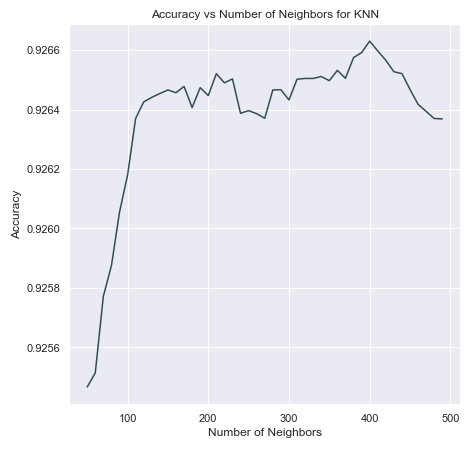
\includegraphics[scale=0.65]{knn_tune} \\ 
With 400, we got a model score of 92.663\%. This is about 0.063\% better than with 60 neighbors. A small but reasonable improvement.\\

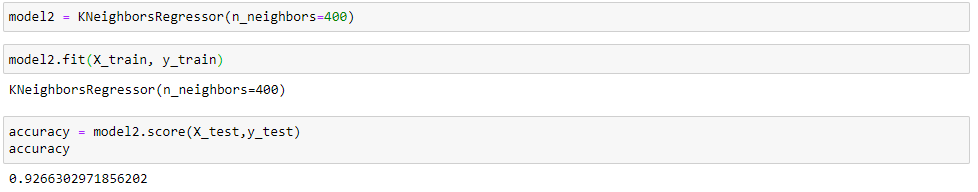
\includegraphics[scale=0.65]{model2} \\ 

\underline{\textbf{Model Tuning: Random Forest}}\\ \\
We can also use GridSearchCV to tune the hyperparameters for the random forest. I ran the gridSearchCV with 5 fold CV. \\
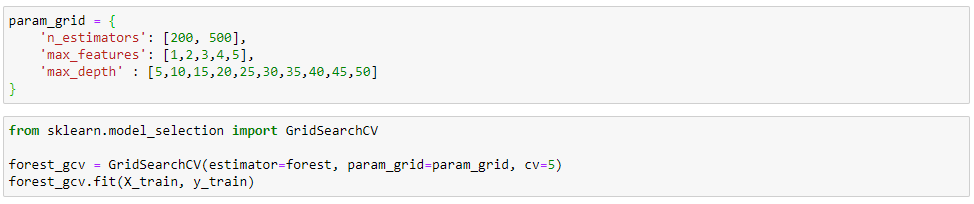
\includegraphics[scale=0.65]{foresty2} \\
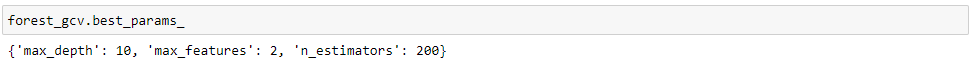
\includegraphics[scale=0.65]{foresty5} \\
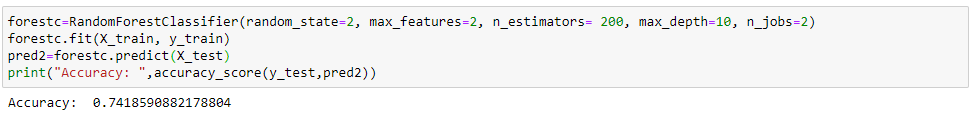
\includegraphics[scale=0.65]{foresty10} \\
However, with the random forest, I didn't really see an improvement after parameter tuning. The grid search already look over 45 minutes to run on my computer. Perhaps with a more robust computer and more values for searching it might be possible to get a better accuracy. However, practically speaking the parameters previously are sufficient. It appears that random forest performs roughly 74-75\% in classifying whether an app will be popular or not. I think the lesson here is sometimes it might not be possible to see an improvement with tuning. 

\underline{\textbf{Further Work}}\\ \\
There's definitely a lot of other things that could be done with the data set. There is a also a user reviews CSV, so it's possible to do some sentiment analysis and natural language processing to find how users feel about apps through their reviews. Another example would be classifying whether a review is fake or not. This data set from Kaggle is a bit old. I think it would be interesting to scrap current app data and analysis it. Especially during this covid time, certain apps have skyrocketed in popularity. It would be interesting to see if it's possible to build a model that can cluster which apps grew the most and which declined the most during the pandemic. Lastly, we can also try building a model that determines the price of an app. Pricing competitively is important to companies and many of companies even have pricing analysts. Overall, this project was fun and there's certainly a lot of further exploration that can be done. With a more powerful computer, it's possible to analysis a bigger data set of apps.

\end{document}




